\documentclass{jlreq}

\usepackage{amsmath}
\usepackage{bm}
\usepackage{fancyhdr}
\usepackage{float}
\usepackage{graphicx}
\usepackage{physics}
\usepackage{siunitx}

\numberwithin{equation}{section}

\pagestyle{fancy}
\fancyhf{}
\fancyhead[R]{\thepage}

\begin{document}

\tableofcontents
\clearpage

\section{実験項目}
% ここに項目を記入
\begin{enumerate}
  \item 理論値を計算するLCR回路の抵抗とキャパシタとインダクタのパラメータを,減衰係数$\zeta$が$\sqrt{2}/6 < \zeta < \sqrt{2}/3$を満たすようにそれぞれ決定する.
  \item 実験項目1.で決定したLCR回路について,インディシャル応答と周波数応答の理論値のグラフを作成する.
  \item 実験項目1.で決定したLCR回路で二次遅れ要素を作成し,インディシャル応答を測定してそのグラフを作成する.
  \item LCR回路の周波数応答を測定してそのボード線図を作成する.
\end{enumerate}

\section{目的}
\subsection{2週目}
LCR回路のインディシャル応答を調べ,時間応答特性について検討する.

\subsection{3週目}
LCR回路の周波数応答を測定してボード線図を作成し,理論値と実測値のグラフの比較を行う.

\section{使用するソフトと部品}
\begin{itemize}
  \item Excel
  \item $33\si{\Omega}$の抵抗
  \item $2.2\si{\micro F}$のコンデンサ
  \item $30\si{\milli\henry}$のコイル
  \item ジャンパーワイヤー
  \item ブレッドボード
  \item Analog Discovery
  \item WaveForms
\end{itemize}

\section{結果}
今回の測定ではオペアンプは用いていない.
上記の抵抗,コンデンサ,コイルを用いたときの,折れ点角周波数$\omega_n$と減衰係数$\zeta$,位相差$\phi$,共振値$M_p$,共振角周波数$\omega_p$の理論値を表\ref{tab:each_theo}に示す.
\begin{table}[H]
  \centering
  \caption{$R=33[\si{\Omega}], C=2.2[\si{\micro F}], L=30[\si{\milli\henry}]$のときの諸理論値}
  \begin{tabular}{|c|c|c|c|c|}
    \hline
    $\omega_n[\si{rad\per\sec}]$ & $\zeta$ & $\phi[\si{rad}]$ & $M_p$  & $\omega_p[\si{rad\per\sec}]$ \\
    \hline
    3892.4                       & 0.37679 & 1.1845           & 1.4326 & 3293.8                       \\
    \hline
  \end{tabular}
  \label{tab:each_theo}
\end{table}

\subsection{インディシャル応答の測定}
LCR回路のインディシャル応答の理論値と実測値は図\ref{fig:lcr_indicial_without_opamp}のようになった.
\begin{figure}[H]
  \centering
  \includegraphics[width=\textwidth]{assets/lcr_indicial_without_opamp.png}
  \caption{LCR回路のインディシャル応答の比較図}
  \label{fig:lcr_indicial_without_opamp}
\end{figure}

このとき,立ち上がり時間と行き過ぎ量の理論値と実測値は表\ref{tab:rise_time_and_over_excessive_amount}のように求まった.
\begin{table}[H]
  \centering
  \caption{立ち上がり時間と行き過ぎ量の比較}
  \begin{tabular}{|c|c|c|}
    \hline
    ~                   & 理論値     & 実測値     \\
    \hline
    立ち上がり時間(sec) & 0.00036618 & 0.00049542 \\
    \hline
    行き過ぎ量(V)       & 0.27860    & 0.14327    \\
    \hline
  \end{tabular}
  \label{tab:rise_time_and_over_excessive_amount}
\end{table}

\subsection{周波数応答の測定}
LCR回路の周波数応答の実測値を表\ref{tab:freq_react}に示す.
\begin{table}[H]
  \centering
  \caption{LCR回路の周波数応答の測定値}
  \begin{tabular}{|r|r|r|}
    \hline
    角周波数($\si{rad\per\sec})$ & ゲイン$G_{dB}(\omega)$(dB) & 位相差\angle{G(jw)}($\si{\degree}$) \\
    \hline
    62.8                         & -0.0328                    & -0.539                              \\ \hline
    628.3                        & 0.1077                     & -6.155                              \\ \hline
    1256.6                       & 0.5266                     & -13.500                             \\ \hline
    1884.9                       & 1.2177                     & -20.869                             \\ \hline
    2513.2                       & 2.1043                     & -31.764                             \\ \hline
    3141.5                       & 2.4947                     & -48.063                             \\ \hline
    3392.9                       & 3.1647                     & -60.697                             \\ \hline
    3455.7                       & 3.2261                     & -61.908                             \\ \hline
    3518.5                       & 3.2226                     & -62.756                             \\ \hline
    3769.9                       & 3.1563                     & -70.632                             \\ \hline
    4084.0                       & 2.8176                     & -87.002                             \\ \hline
    4398.2                       & 2.2729                     & -91.028                             \\ \hline
    5026.5                       & 0.4463                     & -110.571                            \\ \hline
    6283.1                       & -3.3288                    & -128.571                            \\ \hline
    15707.9                      & -20.3920                   & -159.487                            \\ \hline
    18849.5                      & -23.3700                   & -164.051                            \\ \hline
  \end{tabular}
  \label{tab:freq_react}
\end{table}

理論値と実測値を比較したボード線図を図\ref{fig:bode_plot}に示す.
\begin{figure}[H]
  \centering
  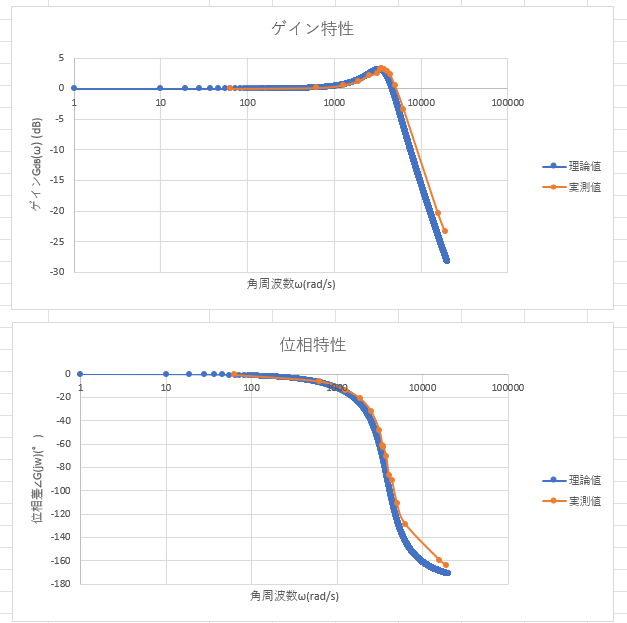
\includegraphics[width=\textwidth]{assets/bode_plot.png}
  \caption{ボード線図}
  \label{fig:bode_plot}
\end{figure}

\section{考察}
\subsection{実験項目3.について}
\subsubsection{インディシャル応答の測定値と実測値の比較} \label{sec:discussion_indicial_comp}
図\ref{fig:lcr_indicial_without_opamp}から,理論値に比べて実測値は電圧の最大値が低く,一定に落ち着くまでの曲線の振動が少なくなだらかである.
これは,実際に用いた抵抗の内部抵抗によってエネルギーの一部が熱として消えてしまい,それによって回路の減衰係数が増加して過渡応答時の振幅が抑制されたと考えられる.

\subsubsection{立ち上がり時間と行き過ぎ量の理論値と実測値の比較}
表\ref{tab:rise_time_and_over_excessive_amount}より,立ち上がり時間の実測値は理論値と比べて遅く,行き過ぎ量の実測値は理論値と比べて小さくなっている.
行き過ぎ量の違いに関しては考察\ref{sec:discussion_indicial_comp}で上げたことが要因として考えられる.一方,立ち上がりに関しては初速は実測値の方が大きいが,
まもなく理論値に追い抜かれてしまう.これに関しても考察\ref{tab:rise_time_and_over_excessive_amount}で上げられたことが要因として考えられ,結果的に立ち上がり時間が理論値と比べて遅くなっている.

\subsection{実験項目4.について}
\subsubsection{周波数応答の測定値と理論値の比較}
図\ref{fig:bode_plot}から,角周波数が高くなるにつれてゲイン特性と位相特性の実測値と理論値とのずれが大きくなっていくことが分かる.
これは,電源ノイズなどの測定環境で発生するノイズが高周波数帯の入力信号と干渉してしまうことにより,ずれが生じてしまったと考えられる.

\subsubsection{折れ点周波数,共振値,共振周波数の理論値と実測値の比較}
周波数応答の測定値から求めた折れ点角周波数,共振値,共振周波数と理論値を表\ref{fig:phase_react_comp}にまとめた.なお,共振値の理論値は単位をdBに変換して計算しており,折れ点周波数の実測値は
位相差が$-90\si{\degree}$に最も近くなるときの周波数の値とした.
\begin{table}[H]
  \centering
  \caption{折れ点周波数,共振値,共振周波数の比較}
  \begin{tabular}{|r|r|r|r|}
    \hline
    ~      & 折れ点周波数($\si{rad\per\sec}$) & 共振値(dB) & 共振周波数($\si{rad\per\sec}$) \\
    \hline
    理論値 & 3892.4                           & 3.1223     & 3293.8                         \\
    \hline
    実測値 & 4398.2                           & 3.2261     & 3455.7                         \\
    \hline
  \end{tabular}
  \label{fig:phase_react_comp}
\end{table}

表\ref{fig:phase_react_comp}から,折れ点周波数と共振値,共振周波数の全てにおいて,理論値よりも実測値の方が大きい値をとっていることが分かる.
共振値を求める式は
\begin{equation}
  M_p = \frac{1}{2\zeta\sqrt{1-\zeta^2}}
\end{equation}
であり,両辺を$\zeta$で微分すると,
\begin{equation}
  M_p' = \frac{2\zeta^2-1}{2\zeta^2(1-\zeta^2)^{\frac{3}{2}}}
\end{equation}
となり,$0 < \zeta < \frac{1}{\sqrt{2}}$のとき単調減少となる.

また,共振角周波数については
\begin{equation}
  \omega_p = \omega_n \sqrt{1-2\zeta^2}
\end{equation}
であることから,$0 < \zeta < \frac{1}{\sqrt{2}}$のとき単調減少となる.

したがって,共振値と共振角周波数の実測値が理論値よりも高くなったということから,高周波数の信号を入力に与えたときのLCR回路の減衰係数が減少したことが分かる.
減衰係数は$\zeta = \frac{R}{2} \sqrt{\frac{C}{L}}$で表されるため,考えられる原因としては高周波数の信号の負荷によってキャパシタンスの減少やインダクタンスの増加が起きてしまうことなどが挙げられる.

\section{問題の解答}
\subsection*{課題4.5.1}
実験テキストのボード線図を確認すると,比較的低い周波数の正弦波を入力としたときにはゲインが$0 \si{\decibel}$で一定となっており,これは入出力で振幅に変化が見られないことを意味する.
また位相に関しても,周波数が比較的低い場合は$0 \si{\degree}$近辺のなだらかな曲線となっており,入出力で位相のずれが小さいと考えられる.

\subsection*{課題4.5.2}
実験テキストのボード線図を確認すると,比較的高い周波数の正弦波を入力としたときにはゲインが負の方向に発散しており,入力に対する出力の振幅がますます小さくなることを意味する.
また位相に関しても,周波数が比較的高い場合は$-90 \si{\degree}$に限りなく近くなるため,入力に対する出力の位相はほぼ$-90 \si{\degree}$となる.

\begin{thebibliography}{9}
  \item シリアーラヤ パノット.プロジェクト実習Ⅰ エレクトロニクス基礎 実験テキスト.京都工芸繊維大学,2024年
\end{thebibliography}

\end{document}